\chapter{Data structure description language}\label{sec:dsdl}

The data structure description language, or \emph{DSDL}, is a simple domain-specific language designed for
defining compound data types.
The defined data types are used for exchanging data between UAVCAN nodes via one of the standard UAVCAN
transport protocols\footnote{The standard transport protocols are documented in chapter \ref{sec:transport_layer}.
UAVCAN doesn't prohibit users from defining their own application-specific transports as well,
although users doing that are likely to encounter compatibility issues and possibly a suboptimal
performance of the protocol.}.

\section{Architecture}

\subsection{General principles}

In accordance with the UAVCAN architecture, DSDL allows users to define data types of two kinds:
message types and service types.
Message types are used to exchange data over publish-subscribe one-to-many message links identified by subject-ID,
and service types are used to perform request-response one-to-one exchanges (like RPC) identified by service-ID.
A message data type defines one data schema of the message object,
and a service data type contains two independent data schema definitions:
one of them applies to the request object (transferred from client to server),
and the other applies to the response object (transferred from the server back to the client).

Following the deterministic nature of UAVCAN, the size of a serialized representation of any
message or service object is bounded within statically known limits.
Variable-size entities always have a fixed size limit defined by the data type designer.

DSDL definitions are strongly statically typed.

DSDL provides well-defined means of data type versioning, which enable data type maintainers to introduce changes
to released data types while ensuring backward compatibility with fielded systems.

DSDL is designed to support extensive static analysis. Important properties of data type definitions such as
backward binary compatibility and data field layouts can be checked and validated by automatic software tools
before the systems utilizing them are fielded.

DSDL definitions can be used to automatically generate serialization (and deserialization) source code
for any data type in a target programming language.
A tool that is capable of generating serialization code based on a DSDL definition is called a \emph{DSDL compiler}.
More generically, a software tool designed for working with DSDL definitions is called a \emph{DSDL processor}.

\subsection{Data types and namespaces}

Every data type is located inside a \emph{namespace}.
Namespaces may be included into higher-level namespaces, forming a tree hierarchy.

A namespace that is at the root of the tree hierarchy (i.e., not nested within another one)
is called a \emph{root namespace}.
A namespace that is located inside another namespace is called a \emph{nested namespace}.

A data type is uniquely identified by its namespaces and its \emph{short name}.
The short name of a data type is the name of the type itself excluding the containing namespaces.

A \emph{full name} of a data type consists of its short name and all of its namespace names.
The short name and the namespace names included in a full name are called \emph{name components}.
Name components are ordered: the root namespace is always the first component of the name,
followed by the nested namespaces, if there are any, in the order of their nesting;
the short name is always the last component of the full name.
The full name is formed by joining its name components via the ASCII dot character ``\verb|.|'' (ASCII code 46).

A \emph{full namespace} name is the full name without the short name and its component separator.

A \emph{sub-root namespace} is a nested namespace that is located immediately under its root namespace.
Data types that reside directly under their root namespace do not have a sub-root namespace.

The name structure is illustrated on the figure \ref{fig:dsdl_data_type_name_structure}.

\begin{figure}[H]
    $$
    \overbrace{
        \underbrace{
            \underbrace{\texttt{\huge{uavcan}}}_{\substack{\text{root} \\ \text{namespace}}}%
            \texttt{\huge{.}}%
            \underbrace{\texttt{\huge{node}}}_{\substack{\text{nested, also} \\ \text{sub-root} \\ \text{namespace}}}%
            \texttt{\huge{.}}%
            \underbrace{\texttt{\huge{port}}}_{\substack{\text{nested} \\ \text{namespace}}}%
        }_{\text{full namespace}}%
        \texttt{\huge{.}}%
        \underbrace{\texttt{\huge{GetInfo}}}_{\text{short name}}
    }^{\text{full name}}
    $$
    \caption{Data type name structure.\label{fig:dsdl_data_type_name_structure}}
\end{figure}

Data type names are case-sensitive.
However, data type names that differ only in letter case are not permitted\footnote{%
Because that may cause problems with case-insensitive file systems.}.

A name component consists of alphanumeric ASCII characters (which are: \verb|A-Z|, \verb|a-z|, and \verb|0-9|)
and underscore (``\verb|_|'', ASCII code 95).
An empty string is not a valid name component.
The first character of a name component must not be a digit.
A name component must not match any of the reserved word patterns,
which are listed in the table \ref{table:dsdl_reserved_word_patterns}.

The length of a full data type name must not exceed 50
characters\footnote{This includes the name component separators.}.

Every data type definition is assigned a major and minor version number pair.
In order to uniquely identify a data type definition, its version numbers must be specified.
In the following text, the term \emph{version} without a majority qualifier refers to
a pair of major and minor version numbers.

Valid data type version numbers range from 0 to 255, inclusively.
A data type version where both major and minor components are zero is not allowed.

\subsection{File hierarchy}

DSDL data type definitions are contained in UTF-8 encoded text files with a file name extension \verb|.uavcan|.

One file defines exactly one version of a data type,
meaning that each combination of major and minor version numbers must be unique per data type name.
There may be an arbitrary number of versions of the same data type defined alongside each other,
provided that each version is defined at most once.
Version number sequences can be non-contiguous,
meaning that it is allowed to skip version numbers or remove existing definitions that are neither oldest nor newest.

A data type definition may have an optional fixed port ID\footnote{Chapter \ref{sec:basic_concepts}.} value specified.

The name of a data type definition file is constructed from the following entities
joined via the ASCII dot character ``\verb|.|'' (ASCII code 46), in the specified order:
\begin{itemize}
    \item Fixed port ID in decimal notation, unless a fixed port ID is not provided for this definition.
    \item Short name of the data type (mandatory, always non-empty).
    \item Major version number in decimal notation (mandatory).
    \item Minor version number in decimal notation (mandatory).
    \item File name extension ``\verb|uavcan|'' (mandatory).
\end{itemize}

\begin{figure}[H]
    $$
    \overbrace{%
        \underbrace{\texttt{\huge{432}}}_{\substack{\text{fixed} \\ \text{port ID}}}%
        \texttt{\huge{.}}%
    }^{\text{optional}}%
    \overbrace{%
        \underbrace{\texttt{\huge{GetInfo}}}_{\substack{\text{short name}}}%
        \texttt{\huge{.}}%
        \underbrace{\texttt{\huge{1.0}}}_{\substack{\text{version} \\ \text{numbers}}}%
        \texttt{\huge{.}}%
        \underbrace{\texttt{\huge{uavcan}}}_{\text{file extension}}%
    }^{\text{mandatory}}
    $$
    \caption{Data type definition file name structure.\label{fig:dsdl_definition_file_name_structure}}
\end{figure}

DSDL namespaces are represented as directories, where one directory defines exactly one namespace, possibly nested.
The name of the directory defines the name of its data type name component.
A directory defining a namespace will always define said namespace in its entirety,
meaning that the contents of a namespace cannot be spread across different directories sharing the same name.
One directory cannot define more than one level of
nesting\footnote{For example, ``\texttt{foo.bar}'' is not a valid directory name.
The valid representation would be ``\texttt{bar}'' nested in ``\texttt{foo}''.}.

An example DSDL directory structure is shown on the figure \ref{fig:dsdl_definition_file_name_structure}.

\begin{figure}[H]
    \begin{tabu}{|l|X|} \hline
        \rowfont{\bfseries}
        Directory tree & Entry description \\\hline

        \texttt{vendor\_x/} &
        Root namespace \texttt{vendor\_x}. \\\cline{2-2}

        \texttt{\qquad{}foo/} &
        Nested namespace (also sub-root) \texttt{vendor\_x.foo}. \\\cline{2-2}

        \texttt{\qquad{}\qquad{}100.Run.1.0.uavcan} &
        Data type definition v1.0 with fixed service ID 100. \\\cline{2-2}

        \texttt{\qquad{}\qquad{}100.Status.1.0.uavcan} &
        Data type definition v1.0 with fixed subject ID 100. \\\cline{2-2}

        \texttt{\qquad{}\qquad{}ID.1.0.uavcan} &
        Data type definition v1.0 without fixed port ID. \\\cline{2-2}

        \texttt{\qquad{}\qquad{}ID.1.1.uavcan} &
        Data type definition v1.1 without fixed port ID. \\\cline{2-2}

        \texttt{\qquad{}\qquad{}bar\_42/} &
        Nested namespace \texttt{vendor\_x.foo.bar\_42}. \\\cline{2-2}

        \texttt{\qquad{}\qquad{}\qquad{}101.List.1.0.uavcan} &
        Data type definition v1.0 with fixed service ID 101. \\\cline{2-2}

        \texttt{\qquad{}\qquad{}\qquad{}102.List.2.0.uavcan} &
        Data type definition v2.0 with fixed service ID 102. \\\cline{2-2}

        \texttt{\qquad{}\qquad{}\qquad{}ID.1.0.uavcan} &
        Data type definition v1.0 without fixed port ID. \\\hline
    \end{tabu}
    \caption{DSDL directory structure example.}\label{fig:dsdl_directory_structure_example}
\end{figure}

\subsection{Elements of data type definition}

A data type definition file contains an exhaustive description of a particular version of the said data type in the
\emph{data structure description language} (DSDL).
As explained above, one data type definition contains either one or two data schema definitions,
for message types and service types, respectively.

The term \emph{attribute} is used to refer to either a field (including padding fields) or a constant
associated with a particular object or type.

A data schema definition contains an ordered, possibly empty collection of \emph{fields} and/or
unordered, possibly empty collection of \emph{constants}.
A data schema may describe either a \emph{structure object} or a \emph{tagged union object}.
The value of a structure object is a function of the values of all of its fields.
A tagged union object is formed from at least two fields,
but it is capable of holding exactly one field at any given time.
The value of a tagged union object is a function of which field it is holding at the moment and the value of said field.

A field represents a named dynamically assigned value of a statically defined type
that can be exchanged over the network as a member of its containing object.
A padding field is a special kind of field which is used for data alignment purposes;
such fields are not named.

A constant represents a named statically defined value of a statically defined type.
Constants are never exchanged over the network, since they are assumed to be known to all involved nodes
by virtue of them sharing the same static definition of the data type.

Constant values are defined via \emph{DSDL expressions},
which are evaluated at the time of DSDL definition processing.
There is a special category of types called \emph{expression types},
instances of which are used only during expression evaluation
and cannot be exchanged over the network.

Data type definitions can also contain various auxiliary elements reviewed later,
such as deprecation markers (notifying its users that the data type is no longer recommended for new designs)
or assertions (special statements introduced by data type designers
which are statically validated by DSDL processing tools).

\subsection{Serialization}

Every object that can be exchanged between UAVCAN nodes has a well-defined \emph{serialized representation}.
The value and meaning of an object can be unambiguously recovered from its serialized representation,
provided that the type of the object is known.

\label{sec:dsdl_bit_length_set}
A serialized representation is a sequence of binary digits (bits);
the number of bits in a serialized representation is called its \emph{bit length}.
A \emph{bit length set} of a data schema refers to the set of bit length values of all possible
serialized representations of objects implementing the schema.

\section{Grammar}

\subsection{Formal definition}

This section contains the formal definition of the DSDL grammar.
Its notation is introduced beforehand.

\subsubsection{Notation}

The notation used in the following definition is a modified ISO/IEC 14977 extended Backus--Naur
form\footnote{This notation is a subset of the notation defined in a Python parsing library titled Parsimonious.
Parsimonious is an MIT-licensed software product authored by Erik Rose;
its sources are available at \url{https://github.com/erikrose/parsimonious}.}.
The rule definition patterns are specified in the table \ref{table:dsdl_grammar_definition_notation}.

\begin{table}[hbtp]
    \begin{UAVCANSimpleTable}{Notation used in the formal grammar definition}{|l X|}
        \label{table:dsdl_grammar_definition_notation}
        Pattern & Description \\

        \texttt{"korovan"} &
        Denotes a terminal string of ASCII characters.
        The string is case-sensitive. \\

        \emph{(space)} &
        Concatenation.
        E.g., ``\texttt{korovan paukan excavator}'' matches a sequence where the specified tokens
        appear in the defined order. \\

        \texttt{korovan / paukan / excavator} &
        Alternatives.
        The leftmost matching alternative is accepted. \\

        \texttt{korovan?} &
        Optional greedy match. \\

        \texttt{paukan*} &
        Zero or more expressions, greedy match. \\

        \texttt{excavator+} &
        One or more expressions, greedy match. \\

        \texttt{\textasciitilde{}r"regex-pattern"} &
        An IEEE POSIX Extended Regular Expression pattern defined between the double quotes.
        The expression operates on the ASCII character set and is always case-sensitive.
        ASCII escape sequences ``\texttt{\textbackslash{}r}'', ``\texttt{\textbackslash{}n}'', and
        ``\texttt{\textbackslash{}t}'' are used to denote ASCII carriage return (code 13),
        line feed (code 10), and tabulation (code 9) characters, respectively. \\

        \texttt{\textasciitilde{}r"regex-pattern"} &
        As above, with single quotes instead of double quotes. \\

        \texttt{(korovan paukan)} &
        Parentheses are used for grouping. \\

    \end{UAVCANSimpleTable}
\end{table}

\subsubsection{Definition}

From the top level down to the expression rule, the grammar is a valid regular grammar,
meaning that it can be parsed using standard regular expressions.
The constant expression syntax is modeled after the Python programming language,
and it cannot be described in terms of a regular grammar.

\clearpage\inputminted[fontsize=\scriptsize]{python}{dsdl/grammar.parsimonious}

\section{Data model}

\subsection{Kinds}

All versions of a data type definition must be of the same kind\footnote{%
For example, if a data type version 0.1 is of a message kind, all later versions of it must be messages, too.}.

\subsubsection{Message}

A message data type definition contains the description of the message data structure without any additional entities.
The data structure description may be empty, i.e. it may define no fields or constants.

\subsubsection{Service}

A service data type definition contains the description of two data structures:
the service request structure followed by the service response structure.
The two structures are separated by the service response marker (``\verb|---|'') on a separate line.
Either or both of the structures may be empty.

The presence of the service response marker indicates that the data type definition at hand is of the service kind.
There may be no more than one service response marker in a given definition.

\subsection{Types}

\subsubsection{Void types}

Void types are used for padding purposes.
As will be explained in later sections, it is desirable to align fields at byte boundaries;
void types can be used to facilitate that.

Void-typed fields are set to zero when a data structure is serialized and ignored when it is deserialized.
Void types can be used to reserve space in data type definitions for possible use in later versions of the data type.

The DSDL name pattern for void types is as follows: ``\verb|void[1-9]\d?|'',
where the trailing one- or two-digit integer represents the length of the void field, in bits,
ranging from 1 to 64, inclusive.

\subsubsection{Primitive types}

Primitive types are defined here. They are assumed to be known to DSDL processing tools a priori,
and as such, they need not be defined by the user.
The following text defines DSDL name patterns using the POSIX Extended Regular Expression (ERE) notation.

The hierarchy of primitive types is documented below.

\begin{itemize}
    \item \textbf{Boolean types.} A boolean-typed value represents a variable of the Boolean algebra.
    A Boolean-typed value can have two values: true and false.
    The corresponding DSDL data type name is ``\verb|bool|''.

    \item \textbf{Algebraic types.} Those are types for which conventional algebraic operators are defined.
    \begin{itemize}
        \item \textbf{Integer types} are used to represent signed and unsigned integer values.
        See table \ref{table:dsd_integer_properties}.
        \begin{itemize}
            \item \textbf{Signed integer types.} These are used to represent values which can be negative.
            The corresponding DSDL data type name pattern is ``\verb|int[1-9]\d?|'',
            where the trailing one- or two-digit integer represents the length of the
            encoded representation of the value, in bits, ranging from 2 to 64, inclusive.

            \item \textbf{Unsigned integer types.} These are used to represent non-negative values.
            The corresponding DSDL data type name pattern is ``\verb|uint[1-9]\d?|'',
            where the trailing one- or two-digit integer represents the length of the
            encoded representation of the value, in bits, ranging from 2 to 64, inclusive.
        \end{itemize}

        \item \textbf{Floating point types} are used to approximately represent real values.
        The underlying encoded representation follows the IEEE 754 standard.
        The corresponding DSDL data type name pattern is ``\verb~float(16|32|64)~'', where the trailing
        integer represents the type of the IEEE 754 representation.
        See table \ref{table:dsd_floating_point_properties}.
    \end{itemize}
\end{itemize}

\begin{UAVCANSimpleTable}{Properties of integer types}{|l X l|}
    Category &
    DSDL names &
    Range, $X$ is bit length
    \label{table:dsd_integer_properties} \\

    Signed integers &
    \texttt{int2}, \texttt{int3}, \texttt{int4} \ldots{} \texttt{int62}, \texttt{int63}, \texttt{int64} &
    $\left[-\frac{2^{X}}{2},\frac{2^{X}}{2}-1\right]$ \\

    Unsigned integers &
    \texttt{uint2}, \texttt{uint3}, \texttt{uint4} \ldots{} \texttt{uint62}, \texttt{uint63}, \texttt{uint64} &
    $\left[0,2^{X}-1\right]$ \\
\end{UAVCANSimpleTable}

\begin{UAVCANSimpleTable}{Properties of floating point types}{|X X X X|}
    DSDL name        & Representation    & Approximate epsilon   & Approximate range
    \label{table:dsd_floating_point_properties} \\

    \texttt{float16} & IEEE 754 binary16 & $0.001$               & $\pm{}65504$      \\
    \texttt{float32} & IEEE 754 binary32 & $10^{-7}$             & $\pm{}10^{39}$    \\
    \texttt{float64} & IEEE 754 binary64 & $2 \times{} 10^{-16}$ & $\pm{}10^{308}$   \\
\end{UAVCANSimpleTable}

An exhaustive list of all void and primitive types ordered by bit length is provided below for reference.

\immediate\write18{rm -f ../latex.tmp}
\immediate\write18{../render_list_of_void_and_primitive_types.py > ../latex.tmp}
\immediate\input{../latex.tmp}

\subsubsection{Array types}

\subsubsection{Compound types}

\subsection{Fields}

% padding fields have no name

\subsection{Constants}

\section{Data serialization}\label{sec:dsdl_data_serialization}

\newcommand{\hugett}[1]{\texttt{\huge{#1}}}

\subsection{General principles}

\subsubsection{Design goals}

The main design principle behind the serialized representations described in this section is
the maximization of compatibility with native representations used by currently existing and
likely future computer microarchitectures.
The goal is to ensure that the serialized representations defined by DSDL match internal data representations of
modern computers, so that, ideally, a typical system will not have to perform any data conversion whatsoever while
exchanging data over a UAVCAN network.

\subsubsection{Bit and byte ordering}

The smallest atomic data entity is a bit.
Eight bits form one byte;
within the byte, the bits are ordered so that the most significant bit is considered first (0-th index),
and the least significant bit is considered last (7-th index).

Numeric values consisting of multiple bytes are arranged so that the least significant byte is encoded first;
such format is also known as little-endian.

\begin{figure}[H]
    $$
    \overset{\text{bit index}}{%
        \underbrace{%
            \overset{0}{\hugett{0}}
            \overset{1}{\hugett{1}}
            \overset{2}{\hugett{0}}
            \overset{3}{\hugett{1}}
            \overset{4}{\hugett{0}}
            \overset{5}{\hugett{1}}
            \overset{6}{\hugett{0}}
            \overset{7}{\hugett{1}}
        }_\text{least significant byte}%
    }
    \hugett{\ldots}
    \overset{\text{bit index}}{%
        \underbrace{%
            \overset{0}{\hugett{0}}
            \overset{1}{\hugett{1}}
            \overset{2}{\hugett{0}}
            \overset{3}{\hugett{1}}
            \overset{4}{\hugett{0}}
            \overset{5}{\hugett{1}}
            \overset{6}{\hugett{0}}
            \overset{7}{\hugett{1}}
        }_\text{most significant byte}%
    }
    $$
    \caption{Bit and byte ordering.\label{fig:dsdl_serialization_bit_ordering}}
\end{figure}

\subsubsection{Implicit padding}

Excepting one edge case reviewed below,
serialized representations of DSDL entities never include implicit data padding.
Unaligned data may lead to suboptimal serialization and deserialization performance;
therefore, the data type designer should manually align elements as necessary to prevent performance degradation.
It is guaranteed, however, that unaligned data cannot result in unspecified or otherwise unexpected behavior
of the data handling routines.
The manual approach to data alignment allows the data type designer to trade-off serialization efficiency
over network bandwidth utilization and data transfer latency as necessary without compromising functional safety.

The exceptional edge case mentioned above when implicit padding is introduced is as follows.
Serialized representations of DSDL entities operate at the bit level,
whereas the transport protocols supported by UAVCAN\footnote{As well as the majority of network protocols in general.}
use byte as the smallest atomic data element.
The resulting mismatch of the data granularity levels is resolved by
appending the serialized representation of the top-level composite type object with zero (0) bits
until the length of its bit sequence is an integer multiple of eight (8).
The term \emph{top-level object} denotes an object that is not nested inside another DSDL entity.
In other words, padding bits may only be added before a fully constructed serialized representation is
handed over for transmission over the UAVCAN network
(or any other destination which does not support bit-level data granularity).

Additionally, the transport layer may introduce extra padding at the end of the serialized representation,
as described in relevant sections of chapter \ref{sec:transport_layer};
however, such padding behavior falls outside of the scope of the DSDL specification
as it belongs to the domain of network transports rather than data presentation.

When a serialized representation is deconstructed, the value of the trailing padding bits must be ignored.

\subsection{Void types}\label{sec:dsdl_serialized_void}

The serialized representation of a void-typed field attribute is constructed as a sequence of zero bits.
The length of the sequence equals the numeric suffix of the type name.

When a void-typed field attribute is decoded, the values of respective bits are ignored;
in other words, any bit sequence of correct length is a valid serialized representation
of a void-typed field attribute.
This behavior facilitates usage of void fields as placeholders for non-void fields
introduced in newer versions of the data type (section \ref{sec:dsdl_versioning}).

\begin{remark}
    The following data schema will be serialized as a sequence of three zero bits $000_2$
    (five trailing padding bits not included):
    \begin{minted}{python}
        void3
    \end{minted}
    The following bit sequences are valid serialized representations of the schema:
    $000_2$,
    $001_2$,
    $010_2$,
    $011_2$,
    $100_2$,
    $101_2$,
    $110_2$,
    $111_2$.
\end{remark}

\subsection{Primitive types}

Serialized representations of instances of the primitive type category that are longer than one byte (8 bits)
are constructed as follows.
First, only the least significant bytes that contain the used bits of the value are preserved;
the rest are discarded following the transformation policy selected by the specified cast mode.
Then the bytes are arranged in the least-significant-byte-first order\footnote{Also known as ``little endian''.}.
If the bit width of the value is not an integer multiple of eight (8),
the rightmost byte (i.e., the most significant byte) is shifted left until the most significant bit of the value
is aligned with the most significant bit of the byte.

\begin{remark}
    The value $1110\,1101\,1010_2$ (3802 in base-10) of type \verb|uint12| is encoded as follows.
    The bit sequence is shown in the base-2 system, where bytes (octets) are comma-separated:
    $$
        \overbrace{%
            \underbrace{\hugett{11011010}}_{\substack{\text{Least significant} \\ \text{bits/byte}}}%
            \hugett{,}%
            \underbrace{\hugett{1110}}_{\substack{\text{Most} \\ \text{significant} \\ \text{bits}}}%
        }^{\text{The value }3802_{10}}%
        \underbrace{\hugett{????}}_{\substack{\text{Next object} \\ \text{or zero} \\ \text{padding bits}}}
    $$
\end{remark}

\subsubsection{Boolean types}\label{sec:dsdl_serialized_bool}

The serialized representation of a value of type \verb|bool| is a single bit.
If the value represents falsity, the value of the bit is zero (0); otherwise, the value of the bit is one (1).

\subsubsection{Unsigned integer types}\label{sec:dsdl_serialized_unsigned_integer}

The serialized representation of an unsigned integer value of length $n$ bits
(which is reflected in the numerical suffix of the data type name)
is constructed as if the number were to be written in base-2 numerical system
with leading zeros preserved so that the total number of binary digits would equal $n$.

\begin{remark}
    The serialized representation of integer 123 of type \verb|uint9| is $001111011_2$.
\end{remark}

\subsubsection{Signed integer types}

The serialized representation of a non-negative value of a signed integer type is constructed as described
in section \ref{sec:dsdl_serialized_unsigned_integer}.

The serialized representation of a negative value of a signed integer type is computed by
applying the following transformation:
$$2^n + x$$
where $n$ is the bit length of the serialized representation
(which is reflected in the numerical suffix of the data type name)
and $x$ is the value whose serialized representation is being constructed.
The result of the transformation is a positive number,
whose serialized representation is then constructed as described in section \ref{sec:dsdl_serialized_unsigned_integer}.

The representation described here is widely known as \emph{two's complement}.

\begin{remark}
    The serialized representation of integer -123 of type \verb|int9| is $110000101_2$.
\end{remark}

\subsubsection{Floating point types}

The serialized representation of floating point types follows the IEEE 754 series of standards as follows:

\begin{itemize}
    \item \verb|float16| --- IEEE 754 binary16;
    \item \verb|float32| --- IEEE 754 binary32;
    \item \verb|float64| --- IEEE 754 binary64.
\end{itemize}

\subsection{Array types}

\subsubsection{Fixed-length array types}

Serialized representations of a fixed-length array of $n$ elements of type $T$ and
a sequence of $n$ field attributes of type $T$ are equivalent.

\begin{remark}
    Serialized representations of the following two data schema definitions are equivalent:

    \begin{minted}{python}
        AnyType[3] array
    \end{minted}

    \begin{minted}{python}
        AnyType item_0
        AnyType item_1
        AnyType item_2
    \end{minted}
\end{remark}

\subsubsection{Variable-length array types}

A serialized representation of a variable-length array consists of two segments:
the implicit length field followed by the array elements.

The implicit length field is of an unsigned integer type.
The serialized representation of the implicit length field
is injected in the beginning of the serialized representation of its array.
The bit length of the unsigned integer value is determined as follows:
$$\lceil{}\log_2 (c + 1)\rceil{}$$
where $c$ is the capacity (i.e., the maximum number of elements) of the variable-length array.
The number of elements $n$ contained in the variable-length array is encoded
in the serialized representation of the implicit length field%
\footnote{%
    Seeing as $n \leq c$ always holds, bit sequences where the implicit length field contains values
    greater than $c$ do not belong to the set of serialized representations of the array.
}
as described in section \ref{sec:dsdl_serialized_unsigned_integer}
(including the case where the bit length of the implicit length field is one bit).

The rest of the serialized representation is constructed as if the variable-length array was
a fixed-length array of $n$ elements.

\begin{remark}
    It is recommended to manually align variable-length arrays by prepending them with padding field attributes
    so that the first element is byte-aligned, as that facilitates more efficient serialization and deserialization.

    \begin{minted}{python}
        void2                        # Padding - good practice but not required
        AnyType.1.0[<42] array       # The implicit length field is 6 bits wide
        @assert _offset_.min == 8    # Ensuring that the first element is byte-aligned
    \end{minted}

    If the array contained three elements,
    the resulting set of its serialized representations would be equivalent to that of the following definition:

    \begin{minted}{python}
        void2                        # Padding - good practice but not required
        uint6 implicit_length_field  # Set to 3, because the array contains three elements
        AnyType.1.0 item_0
        AnyType.1.0 item_1
        AnyType.1.0 item_2
    \end{minted}
\end{remark}

\subsection{Composite types}

As explained in the section \ref{sec:dsdl_composite_types}, a data type of the service kind contains
two data schema definitions: one for request object, one for response object.
Unless explicitly specified otherwise, any reference to serialized representations of a service type
implies either or both of its data schema definitions, depending on context.

A serialized representation of an object of a composite type is an ordered set of serialized representations of
its field attribute values joined into a bit sequence.
The ordering of the serialized representations of the field attribute values follows the order
of field attribute declaration.

\begin{remark}
    Consider the following data schema definition,
    where the fields are assigned runtime values shown in the comments:

    \begin{minted}{python}
        #                          decimal           bit sequence   comment
        truncated uint12 first   # +48858     1011_1110_1101_1010   overflow, MSB truncated
        saturated  int3  second  #     -1                     111   two's complement
        saturated  int4  third   #     -5                    1011   two's complement
        saturated  int2  fourth  #     -1                      11   two's complement
        truncated uint4  fifth   #   +136               1000_1000   overflow, MSB truncated
    \end{minted}

    It can be seen that the bit layout is rather complicated because the field boundaries do not align with byte
    boundaries, which makes it a good case study.
    The resulting serialized byte sequence is shown below in the base-2 system,
    where bytes (octets) are comma-separated:
    $$
        \overbrace{\hugett{11011010,1110}}^{\texttt{first}}%
        \underbrace{\hugett{111}}_{\texttt{second}}%
        \overbrace{\hugett{1,011}}^{\texttt{third}}%
        \underbrace{\hugett{11}}_{\texttt{fourth}}%
        \overbrace{\hugett{100,0}}^{\texttt{fifth}}%
        \underbrace{\hugett{???????}}_{\substack{\text{Next object or} \\ \text{zero padding bits}}}
    $$
\end{remark}

\subsubsection{Tagged unions}

Similar to variable-length arrays, a serialized representation of a tagged union consists of two segments:
the implicit \emph{union tag} value followed by the selected field attribute value.

The implicit union tag is an unsigned integer value whose serialized representation
is implicitly injected in the beginning of the serialized representation of its tagged union.
The bit length of the implicit union tag is determined as follows:
$$\lceil{}\log_2 n\rceil{}$$
where $n$ is the number of field attributes in the union, $n \geq 2$.

Each of the tagged union field attributes is assigned an index according to the order of their definition;
the order follows that of the DSDL statements (see section \ref{sec:dsdl_grammar} on statement ordering).
The first defined field attribute is assigned the index 0 (zero),
the index of each following field attribute is incremented by one.

The index of the field attribute whose value is currently held by the tagged union is encoded
in the serialized representation of the implicit union tag%
\footnote{%
    Seeing as $i < n$ always holds, where $i$ is the index of the current field attribute,
    bit sequences where the implicit union tag field contains values
    that are greater than or equal $n$ do not belong to the set of serialized representations of the tagged union.
}
as described in section \ref{sec:dsdl_serialized_unsigned_integer}
(including the case where the bit length of the implicit length field is one bit).

The serialized representation of the implicit union tag is immediately followed by
the serialized representation of the currently selected field attribute value.

\begin{remark}
    Consider the following example:

    \begin{minted}{python}
        @union           # In this case, the implicit union tag is 2 bit wide
        uint16 FOO = 42  # A regular constant attribute
        uint16 a         # Field index 0
        uint8 b          # Field index 1
        uint32 BAR = 42  # Another regular constant attribute
        float64 c        # Field index 2
    \end{minted}

    In order to encode the field \verb|b|, the implicit union tag shall be assigned the value 1.
    The following data schema will have an identical layout:

    \begin{minted}{python}
        uint2 implicit_union_tag  # Set to 1
        uint8 b                   # The actual value
    \end{minted}

    Suppose that the value of \verb|b| is 7.
    The resulting serialized representation is shown below in the base-2 system:
    $$%
    \underbrace{\hugett{01}}_{\substack{\text{union} \\ \text{tag}}}%
    \underbrace{\hugett{00000111}}_{\text{field }\texttt{b}}%
    $$

    It is recommended to manually align tagged unions when they are nested into outer objects by
    prepending them with a padding field attribute so that the value contained in the union is byte-aligned
    after the tag, as that facilitates more efficient serialization and deserialization.
\end{remark}

\begin{remark}
    Let the following data type be defined under the short name \verb|Empty| and version 1.0:

    \begin{minted}{python}
        # Empty. The only valid serialized representation is an empty bit sequence.
    \end{minted}

    Consider the following union schema definition:

    \begin{minted}{python}
        @union
        Empty.1.0 none
        AnyType.1.0 some
    \end{minted}

    The set of serialized representations of the union schema definition given above is equivalent to
    that of the following variable-length array:

    \begin{minted}{python}
        AnyType.1.0[<=1] maybe_some
    \end{minted}
\end{remark}


\section{Data type compatibility and versioning}\label{sec:dsdl_versioning}

\subsection{Rationale}

Data type definitions may evolve over time as they are refined to better address the needs of their applications.
UAVCAN defines a set of rules that allow data type designers to modify and advance their
data type definitions while ensuring backward compatibility and functional safety.

\subsection{Compatibility}

\subsubsection{Bit compatibility}

A data type or schema $A$ is bit-compatible with a data type or schema $B$ if and only if
the set of serialized representations\footnote{The serialization rules are reviewed
in detail in the section \ref{sec:dsdl_data_serialization}.}
of $A$ is a superset of the set of serialized representations of $B$.

$A$ and $B$ are said to be \emph{mutually bit-compatible} if
their sets of serialized representations are equal.

A \emph{variable-length} data type or schema is a serializable data type or schema
whose set of serialized representations contains bit sequences of different lengths.
Conversely, any data type or schema that is not variable-length is \emph{fixed-length}.

\begin{remark}[breakable]
    The following two definitions are bit-compatible:

    \begin{minted}{python}
        uint32 a
        uint32 b
    \end{minted}

    \begin{minted}{python}
        uint64 c
    \end{minted}

    Consider the following example data type definition; assume that its full data type name is
    \verb|demo.Pair|:

    \begin{minted}{python}
        # demo.Pair
        float16 first
        float16 second
    \end{minted}

    Further, let the following define a data type named \verb|demo.PairVector|:

    \begin{minted}{python}
        # demo.PairVector
        demo.Pair[3] vector
    \end{minted}

    Then the following two definitions are bit-compatible:

    \begin{minted}{python}
        demo.PairVector pair_vector
    \end{minted}

    \begin{minted}{python}
        float16 first_0     # pair_vector.vector[0].first
        float16 second_0    # pair_vector.vector[0].second
        float16 first_1     # pair_vector.vector[1].first
        float16 second_1    # pair_vector.vector[1].second
        float16 first_2     # pair_vector.vector[2].first
        float16 second_2    # pair_vector.vector[2].second
    \end{minted}

    The latter definition in the example above is a flattened unrolled form of the former definition.
    As such, in that particular example, both definitions can be used interchangeably;
    an object serialized using one definition can be deserialized using the other definition.
    However, it is also possible to construct bit-compatible definitions that are not functionally equivalent:

    \begin{minted}{python}
        float16 a
        float32 b
    \end{minted}

    \begin{minted}{python}
        float32 a
        float16 b
    \end{minted}

    Even though the above definitions are bit-compatible, one cannot be substituted with the other.
    The problem of functional equivalency is addressed by the concept of semantic compatibility,
    explored in the section \ref{sec:dsdl_semantic_compatibility}.

    Complicated scenarios are possible when a bit belonging to a primitive-typed field attribute
    is handed over to a constrained field such as an implicit array length field or an implicit union tag field.
    Some interesting examples are shown in the table \ref{table:dsdl_many_compat},
    together with a set of serialized representation patterns.
    Remember that the bits belonging to void-typed field attributes are ignored during deserialization.

    % Please do not remove the hard placement specifier [H], it is needed to keep tables ordered.
    \begin{table}[H]\caption{Complex bit compatibility examples}\label{table:dsdl_many_compat}
        \begin{tabu}{|l|X|X|X|X|X|}
            \hline
            \rowfont{\bfseries}
            &A                  &  B                &  C                &  D                &  E                 \\
            \hline

            \multirow{2}{*}{\textbf{Definition}}
            &\texttt{void1}     &\texttt{bool x}    &\texttt{void1}     &\texttt{bool x}    &\texttt{bool[<5] a} \\
            &\texttt{bool[<3] a}&\texttt{bool[<3] a}&\texttt{bool[<4] a}&\texttt{bool[<4] a}&                    \\
            \hline

            \multirow{8}{*}{%
                \begin{tabular}[x]{@{}l@{}}\textbf{Serialized}\\\textbf{representations}\end{tabular}%
            }
            &\multicolumn{2}{l|}{\texttt{000   }}   &\multicolumn{2}{l|}{\texttt{000    }}  &\texttt{000     } \\
            &\multicolumn{2}{l|}{\texttt{001a  }}   &\multicolumn{2}{l|}{\texttt{001a   }}  &\texttt{001a    } \\
            &\multicolumn{2}{l|}{\texttt{010aa }}   &\multicolumn{2}{l|}{\texttt{010aa  }}  &\texttt{010aa   } \\
            &\multicolumn{2}{l|}{\texttt{      }}   &\multicolumn{2}{l|}{\texttt{011aaa }}  &\texttt{011aaa  } \\
            &\multicolumn{2}{l|}{\texttt{100   }}   &\multicolumn{2}{l|}{\texttt{100    }}  &\texttt{100aaaa } \\
            &\multicolumn{2}{l|}{\texttt{101a  }}   &\multicolumn{2}{l|}{\texttt{101a   }}  &\texttt{        } \\
            &\multicolumn{2}{l|}{\texttt{110aa }}   &\multicolumn{2}{l|}{\texttt{110aa  }}  &\texttt{        } \\
            &\multicolumn{2}{l|}{\texttt{      }}   &\multicolumn{2}{l|}{\texttt{111aaa }}  &\texttt{        } \\
            \hline

            {\begin{tabular}[x]{@{}l@{}}\textbf{Bit-compatible}\\\textbf{with}\end{tabular}}
            &B                  & A                 & A, B, D           & A, B, C           & \emph{(none)}    \\
            \hline
        \end{tabu}
    \end{table}
\end{remark}

\subsubsection{Semantic compatibility}\label{sec:dsdl_semantic_compatibility}

A data type $A$ is semantically compatible with a data type $B$
if an application that correctly uses $A$ exhibits a functionally equivalent behavior to an application
that correctly uses $B$.
The property of semantic compatibility is commutative.

\begin{remark}[breakable]
    Despite using different binary layouts, the following two definitions are semantically compatible
    and also bit-compatible:

    \begin{minted}{python}
        uint16 FLAG_A = 1
        uint16 FLAG_B = 256
        uint16 flags
    \end{minted}

    \begin{minted}{python}
        uint8 FLAG_A = 1
        uint8 FLAG_B = 1
        uint8 flags_a
        uint8 flags_b
    \end{minted}

    Therefore, the definitions can be used interchangeably.
    It should be noted here that due to different set of field and constant attributes,
    the source code auto-generated from the provided definitions may be not drop-in replaceable,
    requiring changes in the application;
    however, source-code-level application compatibility is orthogonal to data type compatibility.
\end{remark}

\subsection{Versioning}

\subsubsection{General assumptions}

The concept of versioning applies only to composite data types.
As such, unless specifically stated otherwise, every reference to ``data type''
in this section implies a composite data type.

A data type is uniquely identified by its full name,
assuming that every root namespace is uniquely named.
There is one or more versions of every data type.

A data type definition is uniquely identified by its full name and the version number pair.
In other words, there may be multiple definitions of a data type differentiated by their version numbers.

\subsubsection{Versioning principles}

Every data type definition has a pair of version numbers ---
a major version number and a minor version number, following the principles of semantic versioning.

For the purposes of the following definitions, a \emph{release} of a data type definition stands for
the disclosure of the data type definition to its intended users or to the general public,
or for the commencement of usage of the data type definition in a production system.

In order to ensure a deterministic application behavior and ensure a robust migration path
as data type definitions evolve, UAVCAN requires that all data type definitions that share the same
full name and the same major version number must be semantically compatible with each other
and mutually bit-compatible with each other.

The versioning rules do not extend to scenarios where the name of a data type is changed,
because that would essentially construe the release of a new data type,
which relieves its designer from all compatibility requirements.
When a new data type is first released,
the version numbers of its first definition must be assigned ``1.0'' (major 1, minor 0).

In order to ensure predictability and functional safety of applications that leverage UAVCAN,
the standard requires that once a data type definition is released,
its DSDL source text, name, version numbers, fixed port-ID, and other properties cannot undergo any
modifications whatsoever, with the following exceptions:
\begin{itemize}
    \item Whitespace changes of the DSDL source text are allowed,
    excepting string literals and other semantically sensitive contexts.

    \item Comment changes of the DSDL source text are allowed as long as such changes
    do not affect semantic compatibility of the definition.

    \item A deprecation marker directive (section~\ref{sec:dsdl_directives}) can be added or removed\footnote{%
    Removal is useful when a decision to deprecate a data type definition is withdrawn.}.
\end{itemize}
Addition or removal of the fixed port identifier is not permitted after a data type definition
of a particular version is released.

Therefore, substantial modifications of released data types are only possible by releasing
new definitions of the same data type.
If it is desired and possible to keep the same major version number for a new definition of the data type,
the minor version number of the new definition shall be one greater than the newest existing minor version
number before the new definition is introduced.
Otherwise, the major version number shall be incremented by one and the minor version shall be set to zero.

An exception to the above rules applies when the major version number is zero.
Data type definitions bearing the major version number of zero are not subjected to any compatibility requirements.
Released data type definitions with the major version number of zero are permitted to change in arbitrary
ways without any regard for compatibility.
It is recommended, however, to follow the principles of immutability, releasing every subsequent definition
with the minor version number one greater than the newest existing definition.

For any data type, there shall be at most one definition per version.
In other words, there must be exactly one or zero definitions
per combination of data type name and version number pair.

All data types under the same name must be also of the same kind.
In other words, if the first released definition of a data type is of the message kind,
all other versions must also be of the message kind.

\subsubsection{Fixed port identifier assignment constraints}

The following constraints apply to fixed port-ID assignments:
\begin{align*}
    \exists P(x_{a.b})                          &\rightarrow \exists P(x_{a.c})
    &\mid&\ b < c;\ x \in (M \cup S)
    \\
    \exists P(x_{a.b})                          &\rightarrow         P(x_{a.b}) =    P(x_{a.c})
    &\mid&\ b < c;\ x \in (M \cup S)
    \\
    \exists P(x_{a.b}) \land \exists P(x_{c.d}) &\rightarrow         P(x_{a.b}) \neq P(x_{c.d})
    &\mid&\ a \neq c;\ x \in (M \cup S)
    \\
    \exists P(x_{a.b}) \land \exists P(y_{c.d}) &\rightarrow         P(x_{a.b}) \neq P(y_{c.d})
    &\mid&\ x \neq y;\ x \in T;\ y \in T;\ T = \left\{ M, S \right\}
\end{align*}
where $t_{a.b}$ denotes a data type $t$ version $a.b$ ($a$ major, $b$ minor);
$P(t)$ denotes the fixed port-ID (whose existence is optional) of data type $t$;
$M$ is the set of message types, and $S$ is the set of service types.

\subsubsection{Non-fixed port identifier assignment recommendations}

For non-fixed port identifiers
it is recommended to ensure that any port identifier of a given kind (subject or service)
is only used with one major version of one data type.

Sharing a port identifier of a given kind with different major versions of the same data type or different data types
is not recommended even if such different types are bit-compatible and semantically compatible
because it may complicate network maintenance and analysis; additionally, it may confuse automated
network analysis software.

The kind is specified above explicitly due to the fact that the sets of subject-ID and service-ID are orthogonal.
In other words,
the numeric value of a port-ID may refer to different data types if they are of different kinds.

\subsubsection{Data type version selection}

DSDL compilers should compile every available data type version separately,
allowing the application to choose from all available major and minor version combination.

When emitting a transfer, the major version of the data type is chosen at the discretion of the application.
The minor version should be the newest available one under the chosen major version.

When receiving a transfer, the node deduces which major version of the data type to use
from its port identifier (either fixed or non-fixed).
The minor version should be the newest available one under the deduced major version\footnote{%
Such liberal minor version selection policy poses no compatibility risks since all definitions under the same
major version are compatible with each other.}.

It follows from the above two rules that when a node is responding to a service request,
the major data type version used for the response transfer shall be the same that is used for the request transfer.
The minor versions may differ, which is acceptable due to the major version compatibility requirements.

\begin{remark}[breakable]
    A simple usage example is provided in this intermission.

    Suppose a vendor named ``Sirius Cybernetics Corporation'' is contracted to design a
    cryopod management data bus for a colonial spaceship ``Golgafrincham B-Ark''.
    Having consulted with applicable specifications and standards, an engineer came up with the following
    definition of a cryopod status message type (named \verb|sirius_cyber_corp.b_ark.cryopod.Status|):

    \begin{minted}{python}
        # sirius_cyber_corp.b_ark.cryopod.Status.0.1

        float16 internal_temperature    # [kelvin]
        float16 coolant_temperature     # [kelvin]

        # Status flags in the lower bits
        uint8 FLAG_COOLING_SYSTEM_A_ACTIVE = 1
        uint8 FLAG_COOLING_SYSTEM_B_ACTIVE = 2
        # Error flags in the higher bits
        uint8 FLAG_PSU_MALFUNCTION = 32
        uint8 FLAG_OVERHEATING     = 64
        uint8 FLAG_CRYOBOX_BREACH  = 128
        # Storage for the above defined flags (this is not the recommended practice)
        uint8 flags
    \end{minted}

    The definition is then deployed to the first prototype for initial laboratory testing.
    Since the definition is experimental, the major version number is set to zero in order to signify the
    tentative nature of the definition.
    Suppose that upon completion of the first trials it is identified that the units must track their power consumption
    in real time for each of the three redundant power supplies independently.

    It is easy to see that the amended definition shown below is neither semantically compatible nor bit-compatible
    with the original definition; however, it shares the same major version number of zero, because the backward
    compatibility rules do not apply to zero-versioned data types to allow for low-overhead experimentation
    before the system is deployed and fielded.

    \begin{minted}{python}
        # sirius_cyber_corp.b_ark.cryopod.Status.0.2

        truncated float16 internal_temperature    # [kelvin]
        truncated float16 coolant_temperature     # [kelvin]

        saturated float32 power_consumption_0     # [watt] Power consumption by the redundant PSU 0
        saturated float32 power_consumption_1     # [watt] likewise for PSU 1
        saturated float32 power_consumption_2     # [watt] likewise for PSU 2

        # Status flags in the lower bits
        uint8 FLAG_COOLING_SYSTEM_B_ACTIVE = 1
        uint8 FLAG_COOLING_SYSTEM_A_ACTIVE = 2
        # Error flags in the higher bits
        uint8 FLAG_PSU_MALFUNCTION = 32
        uint8 FLAG_OVERHEATING     = 64
        uint8 FLAG_CRYOBOX_BREACH  = 128
        # Storage for the above defined flags (this is not the recommended practice)
        uint8 flags
    \end{minted}

    The last definition is deemed sufficient and is deployed to the production system
    under the version number of 1.0: \verb|sirius_cyber_corp.b_ark.cryopod.Status.1.0|.

    Having collected empirical data from the fielded systems, the Sirius Cybernetics Corporation has
    identified a shortcoming in the v1.0 definition, which is corrected in an updated definition.
    Since the updated definition, which is shown below, is mutually semantically
    compatible\footnote{The topic of data serialization is explored in detail in the section
    \ref{sec:dsdl_data_serialization}.}
    with v1.0, the major version number is kept the same and the minor version number is incremented by one:

    \begin{minted}{python}
        # sirius_cyber_corp.b_ark.cryopod.Status.1.1

        saturated float16 internal_temperature    # [kelvin]
        saturated float16 coolant_temperature     # [kelvin]

        float32[3] power_consumption    # [watt] Power consumption by the PSU

        # Error flags (this is the recommended practice)
        bool flag_cryobox_breach
        bool flag_overheating
        bool flag_psu_malfunction

        void3   # Reserved for other flags

        # Status flags (this is the recommended practice)
        bool flag_cooling_system_a_active
        bool flag_cooling_system_b_active
    \end{minted}

    Since the definitions v1.0 and v1.1 are mutually bit-compatible and semantically compatible,
    UAVCAN nodes using either of them can successfully interoperate on the same bus.

    Suppose further that at some point a newer version of the cryopod module,
    equipped with better temperature sensors, is released.
    The definition is updated accordingly to use \verb|float32| for the temperature fields instead of \verb|float16|.
    Seeing as that change breaks the bit compatibility,
    the major version number has to be incremented by one,
    and the minor version number has to be reset back to zero:

    \begin{minted}{python}
        # sirius_cyber_corp.b_ark.cryopod.Status.2.0

        float32 internal_temperature    # [kelvin]
        float32 coolant_temperature     # [kelvin]

        float32[3] power_consumption    # [watt] Power consumption by the PSU

        # Error flags (this is the recommended practice)
        bool flag_cryobox_breach
        bool flag_overheating
        bool flag_psu_malfunction

        void3   # Reserved for other flags

        # Status flags (this is the recommended practice)
        bool flag_cooling_system_a_active
        bool flag_cooling_system_b_active
    \end{minted}

    Nodes using v1.0, v1.1, and v2.0 definitions can still coexist on the same network,
    and they can interoperate successfully as long as they all support at least v1.x or v2.x.

    In general, nodes that need to maximize their compatibility are likely to employ all existing major versions of
    each used data type.
    If there are more than one minor versions available, the highest minor version within the major version should
    be used in order to take advantage of the latest changes in the data type definition.
    It is also expected that in certain scenarios some nodes may resort to publishing the same message type
    using different major versions concurrently to circumvent compatibility issues
    (in the example reviewed here that would be v1.1 and v2.0).
\end{remark}

\section{Application-level conventions}\label{sec:application_conventions}

This section describes a set of high-level conventions designed to enhance compatibility
of applications leveraging UAVCAN.
The conventions described here are not mandatory to follow;
however, every deviation should be justified and documented.

\subsection{Node identifier distribution}

An overview of related concepts is provided in chapter~\ref{sec:basic}.

Valid values of node-ID range from 0 up to a transport-specific upper boundary
which is guaranteed to be above 127 for any transport.

The two uppermost node-ID values are reserved for diagnostic and debugging tools;
these node-ID values should not be used in fielded systems.

\subsection{Timing constraints}

\subsubsection{Recommended message publication timing constraints}

Generally, it is recommended to abort a message transmission if it cannot be completed in 1 second.

It is expected that high-frequency high-priority messages may opt for lower timeout values,
whereas low-priority delayable data may opt for higher timeout values to account for network congestion.
Refer to section~\ref{sec:transport_transfer_priority} on transfer prioritization.

\subsubsection{Recommended service invocation timing constraints}

It is recommended to abort a service transfer transmission if it cannot be completed in 1 second.
It is recommended to stop waiting for a service response if it could not be received in the same amount of time;
upon reaching this condition, the service request operation should be considered unsuccessful.

If the server uses a significant part of the timeout period to process the request,
the client might drop the request before receiving the response.
It is recommended to ensure that the server will be able to process any request in less than 0.5 seconds.

\subsection{Coordinate frames}

UAVCAN follows the conventions that are widely accepted in relevant applications.
Adherence to the coordinate frame conventions described here maximizes compatibility and
reduces the amount of computations for conversions between incompatible coordinate systems and
representations.
It is recognized, however, that some applications may find the advised conventions unsuitable,
in which case deviations are permitted.
Any such deviations shall be explicitly documented.

All coordinate systems defined in this section are right-handed.
If application-specific coordinate systems are introduced, they should be right-handed as well.

\begin{figure}[hbt]
    \centering
    % The source image is released under CC0, public domain, no attribution required:
    % https://commons.wikimedia.org/wiki/File:ECEF_ENU_Longitude_Latitude_relationships.svg
	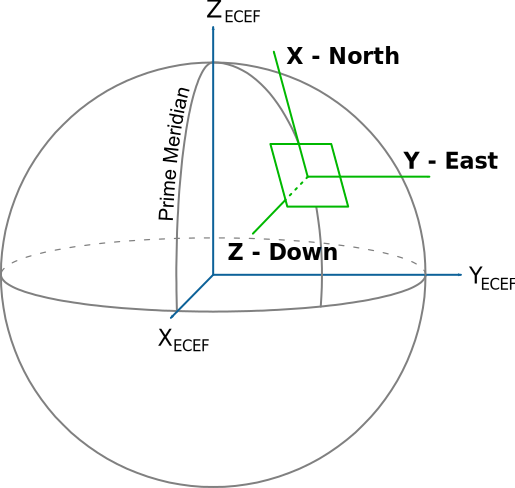
\includegraphics[width=0.45\textwidth]{application/NED_ECEF}
    % The source image is released under CC0, public domain, no attribution required:
    % https://pixabay.com/en/airplane-plane-aircraft-propeller-40374/
    % The final image is drawn by me. The source Inkscape SVG file is located in the same directory.
    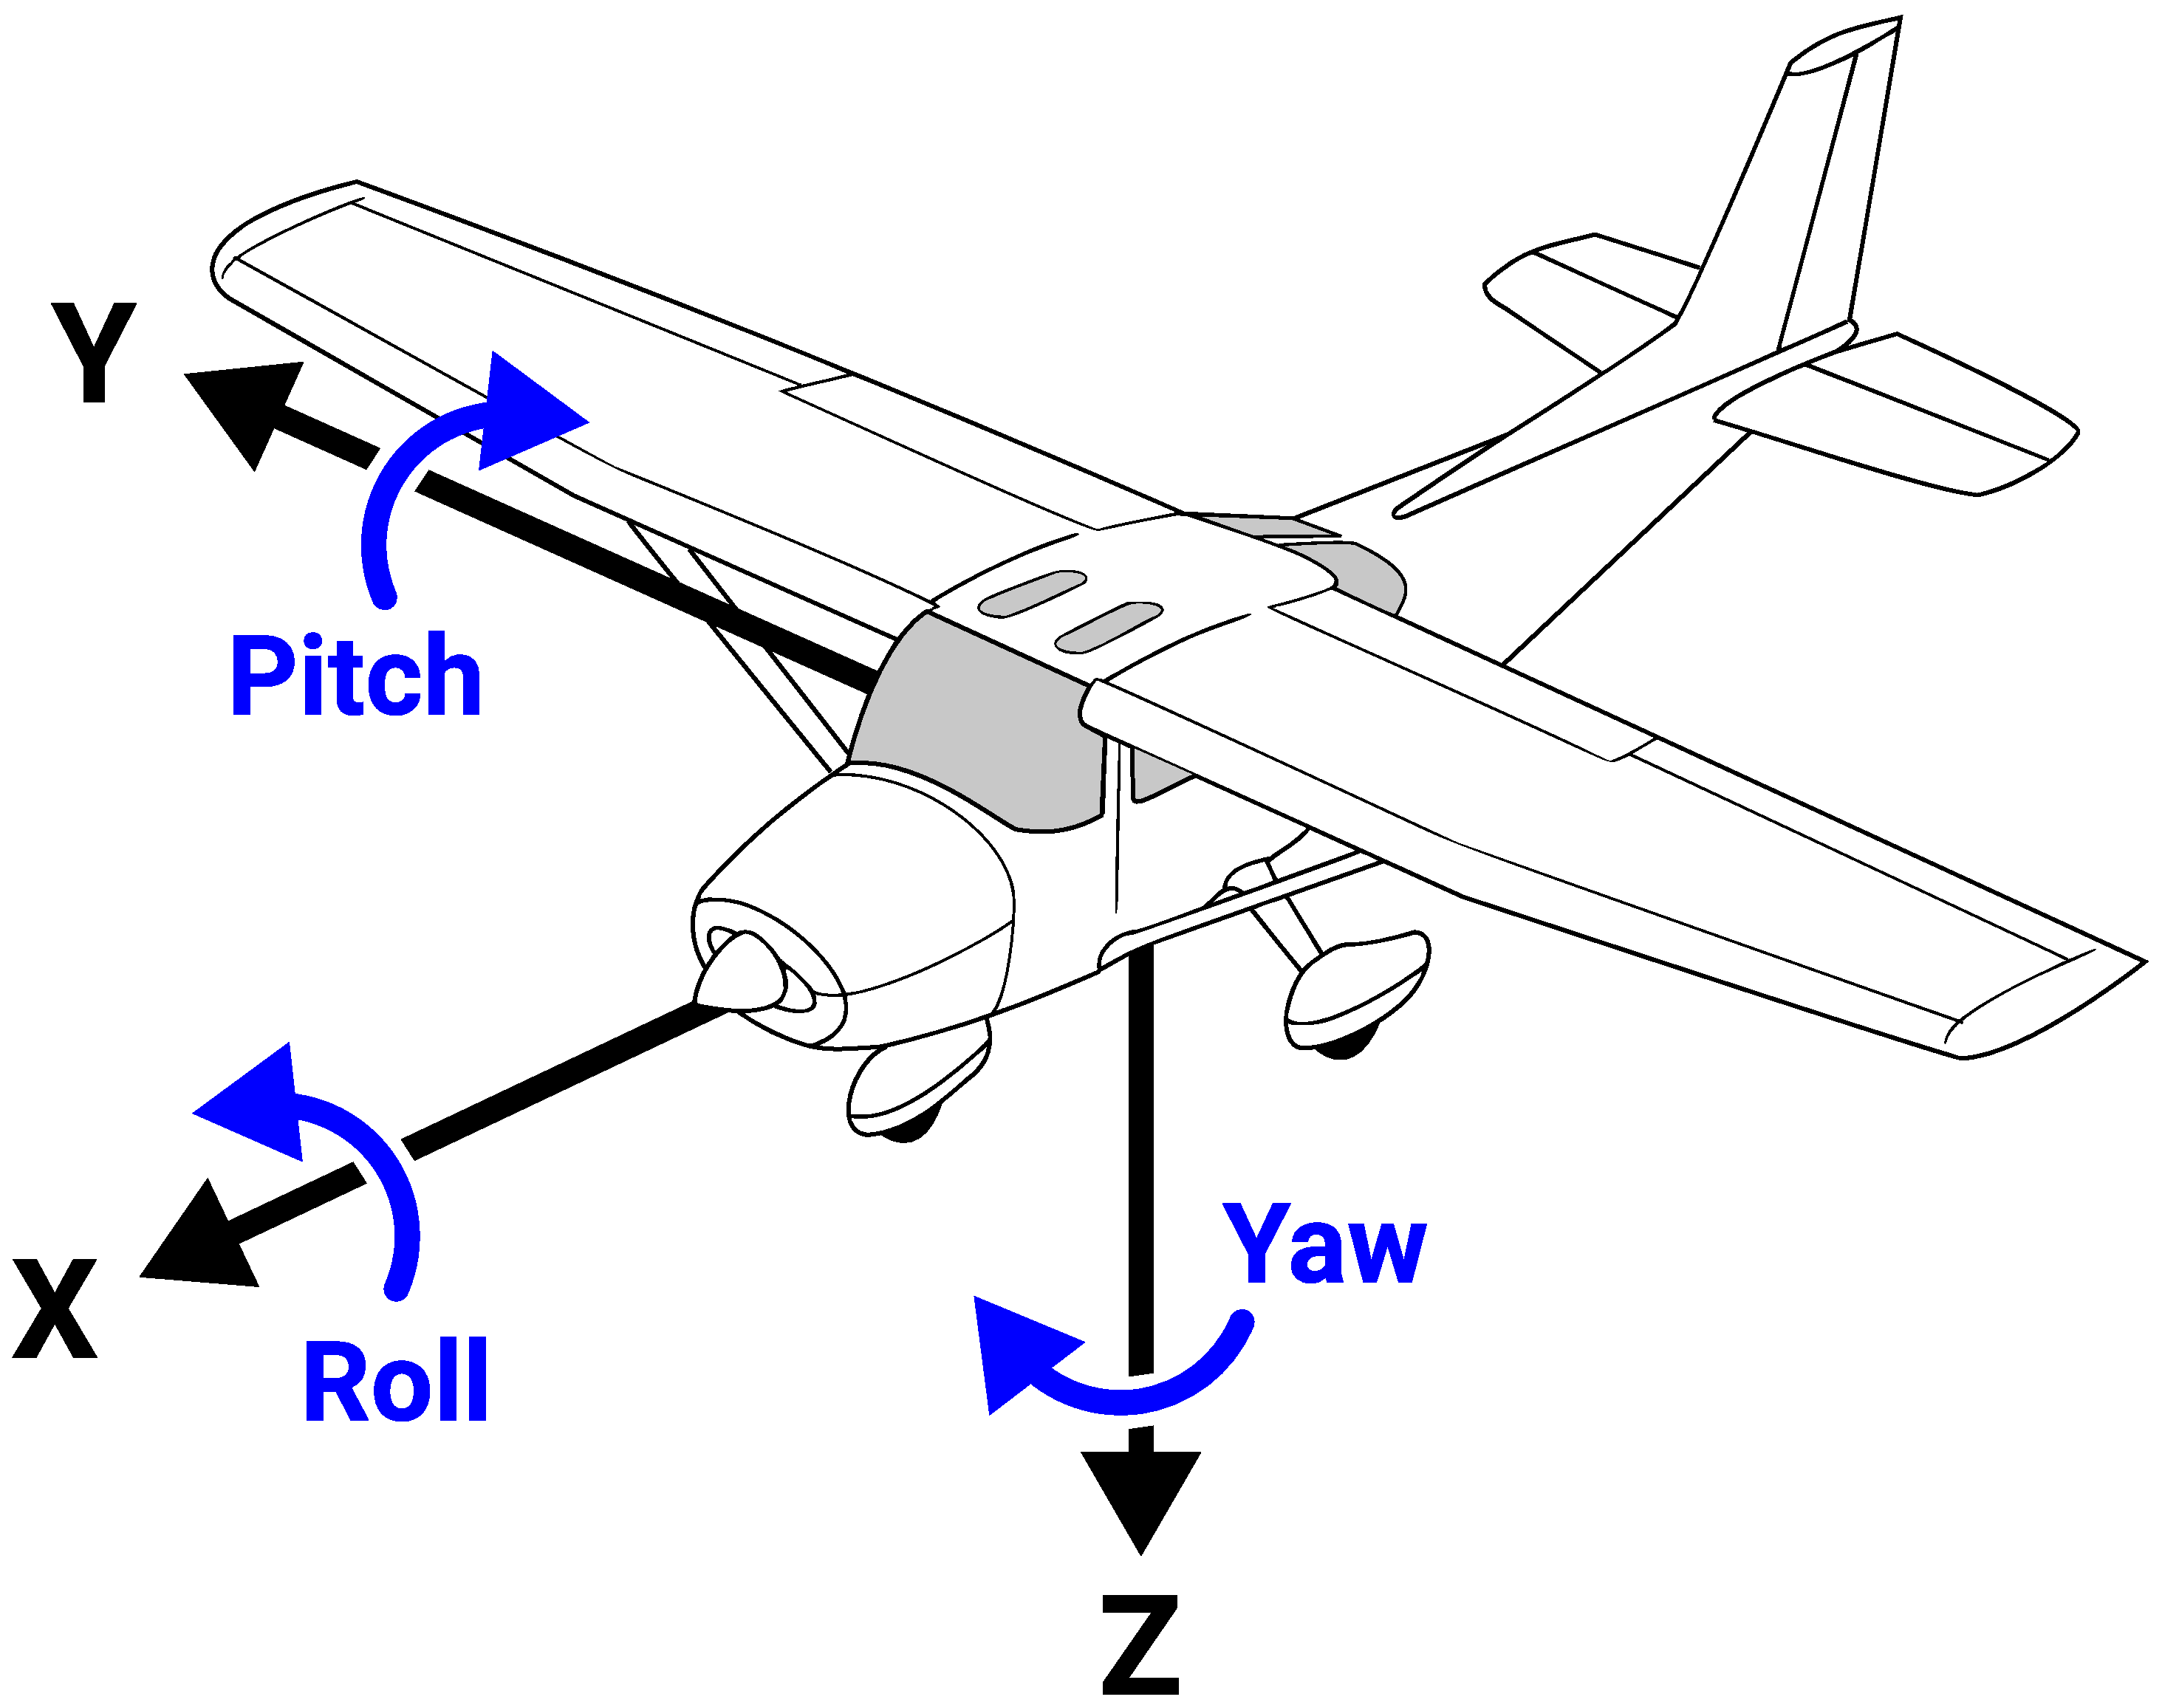
\includegraphics[width=0.45\textwidth]{application/aircraft_principal_axes}
    North-East-Down (NED) frame and body frame conventions. All systems are right-handed.
    \caption{Coordinate frame conventions\label{fig:application_conventions_coordinate_frame}}
\end{figure}

\subsubsection{World frame}

For world fixed frames, the \emph{North-East-Down} (NED) right-handed notation is preferred.
\begin{samepage}
    \begin{description}
        \item[X] --- northward;
        \item[Y] --- eastward;
        \item[Z] --- down.
    \end{description}
\end{samepage}

\subsubsection{Body frame}

In relation to a body, the convention is as defined below, right-handed.
This convention is widely used in aeronautic applications.
\begin{samepage}
    \begin{description}
        \item[X] --- forward;
        \item[Y] --- right;
        \item[Z] --- down.
    \end{description}
\end{samepage}

\subsubsection{Optical frame}

In the case of cameras, the right-handed convention specified below is preferred.
It is widely used in various applications involving computer vision systems.
\begin{samepage}
    \begin{description}
        \item[X] --- right;
        \item[Y] --- down;
        \item[Z] --- towards the scene along the optical axis.
    \end{description}
\end{samepage}

\subsection{Rotation representation}

All applications should represent rotations using quaternions with the elements ordered as follows\footnote{%
    Assuming $w + x\boldsymbol{i} + y\boldsymbol{j} + z\boldsymbol{k}$.
}: W, X, Y, Z.
Other forms of rotation representation should be avoided.

Angular velocities should be represented using the right-handed, fixed-axis (extrinsic) convention:
X (roll), Y (pitch), Z (yaw).

\begin{remark}
    Quaternions are considered to offer the optimal trade-off between bandwidth efficiency,
    computation complexity, and explicitness:
    \begin{itemize}
        \item Euler angles are not self-contained, requiring applications to agree on a particular
              convention beforehand; a convention would be difficult to establish considering different
              demands of various use cases.

        \item Euler angles and fixed axis rotations typically cannot be used for computations directly
              due to angular interpolation issues and singularities; thus, to make use of such
              representations, one often has to convert them to a different form (e.g., quaternion);
              such conversions are computationally heavy.

        \item Rotation matrices are highly redundant.
    \end{itemize}
\end{remark}

\subsection{Matrix representation}

\subsubsection{General}

Matrices should be represented as flat arrays in the row-major order.

\begin{remark}
    $
    \begin{bmatrix}
        x_{11} & x_{12} & x_{13} \\
        x_{21} & x_{22} & x_{23} \\
    \end{bmatrix} \rightarrow \left(x_{11}, x_{12}, x_{13}, x_{21}, x_{22}, x_{23}\right)
    $
\end{remark}

\subsubsection{Square matrices}

There are standard compressed representations of an $n \times n$ square matrix.

An array of size $n^2$ represents a full square matrix.
This is equivalent to the general case reviewed above.

An array of $\frac{(1 + n) n}{2}$ elements represents a symmetric matrix,
where array members represent the elements of the upper-right triangle arranged in the row-major order.
\begin{remark}
    $
    \begin{bmatrix}
        a & b & c \\
        b & d & e \\
        c & e & f \\
    \end{bmatrix} \rightarrow \left(a, b, c, d, e, f\right)
    $

    This form is well-suited for covariance matrix representation.
\end{remark}

An array of $n$ elements represents a diagonal matrix,
where an array member at position $i$ (where $i=1$ for the first element)
represents the matrix element $x_{i, i}$ (where $x_{1, 1}$ is the upper-left element).
\begin{remark}
    $
    \begin{bmatrix}
        a & 0 & 0 \\
        0 & b & 0 \\
        0 & 0 & c \\
    \end{bmatrix} \rightarrow \left(a, b, c\right)
    $
\end{remark}

An array of one element represents a scalar matrix.
\begin{remark}
    $
    \begin{bmatrix}
        a & 0 & 0 \\
        0 & a & 0 \\
        0 & 0 & a \\
    \end{bmatrix} \rightarrow a
    $
\end{remark}

An empty array represents a zero matrix.

\subsubsection{Covariance matrices}

A zero covariance matrix represents an unknown covariance\footnote{%
    As described above, an empty array represents a zero matrix,
    from which follows that an empty array represents unknown covariance.
}.

Infinite error variance means that the associated value is undefined.

\subsection{Physical quantity representation}

\subsubsection{Units}

All units should be SI\footnote{International System of Units.} units (base or derived).
Usage of any other units is strongly discouraged.

When defining data types, fields and constants that represent unscaled quantities in SI units
should not have suffixes indicating the unit, since that would be redundant.

On the other hand, fields and constants that contain quantities in
non-SI units\footnote{E.g., degree Celsius instead of kelvin.}
or scaled SI units\footnote{E.g., microsecond instead of second.}
should be suffixed with the standard abbreviation of the unit\footnote{E.g., kg for kilogram, J for joule.}
and its metric prefix\footnote{E.g., M for mega, n for nano.}
(if any), maintaining the proper letter case of the abbreviation.
In other words, the letter case of the suffix is independent of the letter case of
the attribute it is attached to.

Scaling coefficients should not be chosen arbitrarily;
instead, the choice should be limited to the standard metric prefixes defined by the
International System of Units.

All standard metric prefixes have well-defined abbreviations that are constructed from ASCII characters,
except for one: the micro prefix is abbreviated as a Greek letter ``\textmu{}'' (mu).
When defining data types, ``\textmu{}'' should be replaced with the lowercase Latin letter ``u''.

Irrespective of the suffix, it is recommended to always specify units for every field in the comments.

\begin{remark}
    \begin{minted}{python}
        float16 temperature           # [kelvin] Suffix not needed because an unscaled SI unit is used here.

        uint24 delay_us               # [microsecond] Scaled SI unit, suffix required. Mu replaced with "u".
        uint24 MAX_DELAY_us = 600000  # [microsecond] Notice the letter case.

        float32 kinetic_energy_GJ     # [gigajoule] Notice the letter case.

        float16 estimated_charge_mAh  # [milliampere hour] Scaled non-SI unit. Discouraged, use coulomb.
        float16 MAX_CHARGE_mAh = 1e4  # [milliampere hour] Notice the letter case.
    \end{minted}
\end{remark}

\subsubsection{Enhanced type safety}

In the interest of improving type safety and reducing the possibility of a human error,
it is recommended to avoid reliance on raw scalar types (such as \verb|float32|)
when defining fields containing physical quantities.
Instead, the explicitly typed alternatives defined in the standard DSDL namespace
\DSDLReference{uavcan.si.unit} (also see section~\ref{sec:application_functions_si}) should be used.

\begin{remark}
    \begin{minted}{python}
        float32[4] kinetic_energy                           # [joule] Not recommended.
        uavcan.si.unit.energy.Scalar.1.0[4] kinetic_energy  # This is the recommended practice.
        # Kinetic energy of four bodies.

        float32[3] velocity                                 # [meter/second] Not recommended.
        uavcan.si.unit.velocity.Vector3.1.0                 # This is the recommended practice.
        # 3D velocity vector.
    \end{minted}
\end{remark}

